\cleardoublepage
\section{Lösungsansatz}
In diesem Kapitel wird der von mir implementierte Lösungsansatz vorgestellt. Grundlegend gehe ich zuerst auf die Erweiterung der Simulationsumgebung und die implementierte Transformationskette ein.\\
Danach folgen genauere Ausführungen zu den Kernelementen der Arbeit, der Objekterkennung und dem Schätzverfahren.\\

Ein grundlegender Datentyp, der sich über alle Teile der Arbeit erstreckt, ist durch die Struktur \textit{pointInFrame} [Listing \ref{pointInFrame}] definiert. Diese Struktur bildet einen von der Objekterkennung detektierten Punkt des Objektes mit seiner Position und Orientierung ab. Zudem wird gespeichert, in welchem Referenzframe der Punkt angegeben ist. Neben diesen Positionsdaten sind zudem noch die Gütefaktoren der Objekterkennung angegeben (siehe hierfür Kapitel \ref{sec_learnWeights}).

\begin{lstlisting}[language=Matlab,caption={[Initialisierung der \textit{pointInFrame}-Struktur]Initialisierung der \textit{pointInFrame}-Struktur, die erkannte Punkte in verschiedenen Referenzkoordinatensystemen abbildet.}, label = pointInFrame]
Point_In_Frame = struct;
Point_In_Frame.point = [0 0 0];
Point_In_Frame.direction = 0;
Point_In_Frame.peakheight = 0;
Point_In_Frame.area = 0;
Point_In_Frame.frame = frames.image
Point_In_Frame.numParts = 0;
Point_In_Frame.fitsBorder = false;
Point_In_Frame.relativeCount = 0;
Point_In_Frame.valid = false;
Point_In_Frame.theta = 0;
Point_In_Frame.phi = 0;
\end{lstlisting}

\begin{figure}[H]
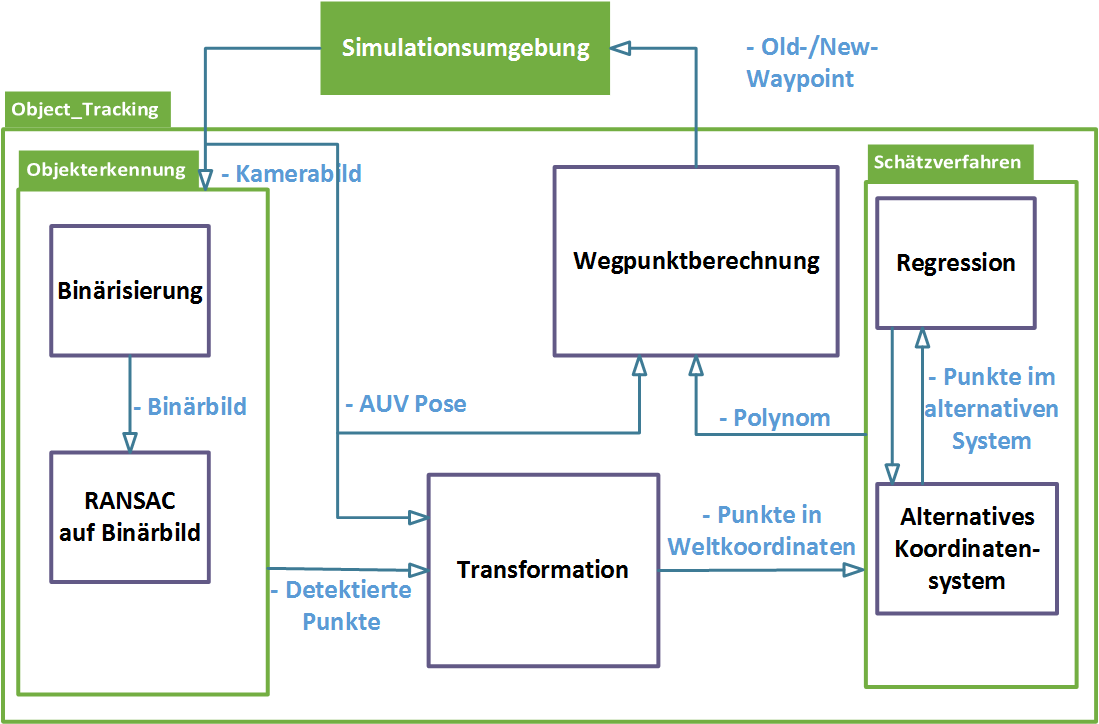
\includegraphics[width=\textwidth]{Systementwurf.png}
\caption[Systementwurf]{Systementwurf der eingesetzten Lösung. Die Simulationsumgebung ist hierbei als \textit{black box} zu betrachten, die das Kamerabild und \gls{auv}-Pose liefert und durch die Wegpunkte für den \gls{lanefollow} gesteuert wird. In dieser Grafik ist der Datenfluss der vier Hauptkomponenten der Arbeit (Objekterkennung, Transformation, Schätzverfahren und Wegpunktberechnung) dargestellt.}
\end{figure}
Die Objekterkennung nutzt das Kamerabild aus der Simulationsumgebung um in zwei Schritten (Binärisierung und \gls{rans}) das Objekt zu detektieren. Die detektierten Punkte werden mithilfe der Information der \gls{auv}-Pose in das globale Weltkoordinatensystem transformiert. Im Schätzverfahren wird das alternative Weltkoordinatensystem geführt, in welchem auch die Regression durchgeführt wird. Mit dem Polynom aus dem Schätzverfahren und der \gls{auv}-Pose werden die Wegpunkte für den \gls{lanefollow} bestimmt.

\subsection{Simulationserweiterung}
\subsubsection{Steuerung}
\label{sec_waypoint}
Wie im Kapitel \ref{sec_auvSimGrundlage} Grundlagen beschrieben, wird in der bestehenden Simulation ein \texttt{\gls{lanefollow}}, der eine Linie zwischen einem \textit{old\_waypoint} und einem\\\textit{new\_waypoint} bildet, verwendet.
Die Schnittstelle zur Steuerung bildet somit die Kombination aus den beiden Wegpunkten. Die Berechnung der Wegpunkte wird auf Basis des Polynoms aus dem Schätzverfahren generiert.\\
Zunächst wird die Position des \gls{auv}s durch die aktuelle Transformationsmatrix in das alternative Weltkoordinatensystem (siehe Absatz \ref{alterWorldCoords}) transformiert. Es wird der, zu dieser Position, nächstgelegene Punkt auf dem Polynom berechnet. Dieser Punkt dient als Zentrum für einen Kreis zur Bestimmung der Wegpunkte. Mithilfe der Kreisgleichung [Gleichung \ref{circEq}] werden die zwei Schnittpunkte des Polynoms mit dem Kreis berechnet. Da durch die Nutzung des alternativen Weltkoordinatensystem sichergestellt wird, dass das \gls{auv} in Richtung der X-Achse fährt, kann problemlos der Schnittpunkt mit höherem $x$-Wert als \textit{next\_waypoint} und dementsprechend der zweite als \textit{old\_waypoint} verwendet werden. Es wird davon ausgegangen, dass bei einem solch kleinen Kreisradius (zwischen 5 und 10 Metern) nicht mehr als zwei Schnittpunkte zwischen Polynom und Kreis vorhanden sind. Sollte dies der Fall sein, wäre das Polynom viel zu stark gekrümmt, um noch verfolgt zu werden. Im Szenario dieser Arbeit gibt es auch keine Objekte, die eine solch starke Krümmung aufweisen.\\
Der letzte Schritt besteht aus der \gls{transform} der Wegpunkte in das reale VRML-Koordinatensystem mithilfe der inversen Transformationsmatrix.
Das Verfahren ist in Abbildung \ref{wpCircle} grafisch dargestellt.

\begin{ownequation}[H]
\begin{equation}
0 = (X_{test}-Center_X)^2+(Y_{test}-Center_Y)^2 - r^2
\end{equation}
\caption[Kreisgleichung zum Test, ob ein Punkt auf einem Kreis liegt.]{Kreisgleichung zum Test ob ein Punkt $X_{test},Y_{test}$ auf einem Kreis liegt. $Center_X$ und $Center_Y$ bilden hierbei den Mittelpunkt eines Kreises mit Durchmesser $r$.}
\label{circEq}
\end{ownequation}

\begin{figure}[H]
\centering
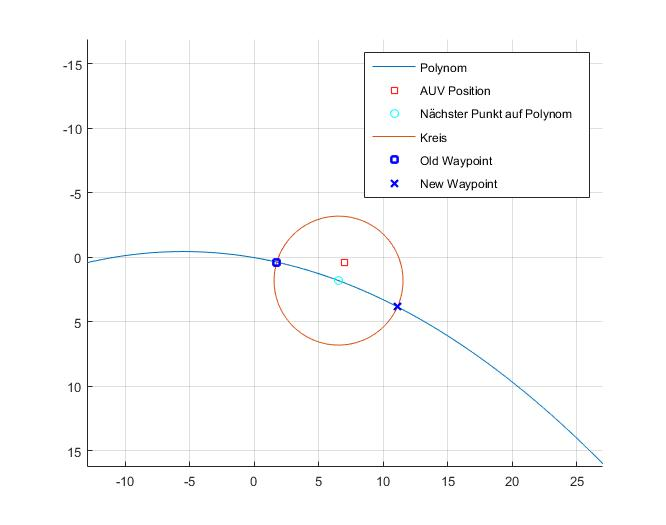
\includegraphics[scale=0.7]{waypointProvier.jpg}
\caption[Verfahren zur Bestimmung der Wegpunkte]{Verfahren zur Bestimmung der Wegpunkte. Der Wegpunkt wird im alternativen Weltkoordinatensystem bestimmt. Hierbei wird ein Kreis um den nächsten Punkt vom \gls{auv} auf dem Polygon bestimmt. Die Schnittpunkte des Kreises bilden die Wegpunkte für die \gls{auv}-Steuerung.}
\label{wpCircle}
\end{figure}
\subsubsection{Kamerabilder}
Da die Simulation in der ursprünglichen Form noch sehr \textit{klinische} Bilder generierte, mussten diese Bilder künstlich verschlechtert und die Sichtverhältnisse eingeschränkt werden, um realistische Eingangsbilder zu erzeugen. In Abbildung \ref{simPics} ist ein ursprüngliches Kamerabild, zwei verschlechterte Bilder und ein sehr stark verschlechtertes Bild zu sehen. Die Testläufe der Arbeit wurden mit den Verschlechterungsgraden aus Abb. \ref{img_badQuali} und \ref{img_testQuali} durchgeführt. Abb. \ref{img_badSeight} zeigt die Sichtbedingungen für Tests mit sehr schlechten Bedingungen.
\begin{figure}[H]
\centering
\begin{tabular}{cc}
\subfloat[Ursprüngliches Bild]{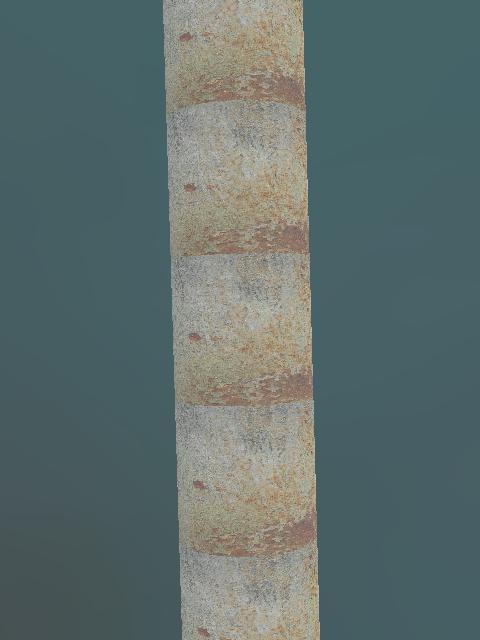
\includegraphics[height=0.25\textheight,width=0.4\textwidth]{/imageProcessing/gradeOptimal.jpg}}&
\subfloat[Bild verschlechtert mit leichter \gls{blur} und geringem Pixelrauschen]{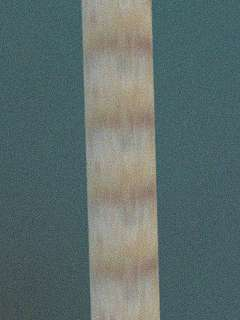
\includegraphics[height=0.25\textheight,width=0.4\textwidth]{/imageProcessing/graeOk.jpg}\label{img_badQuali}}\\
\subfloat[Sichtverhältnisse stark verschlechtert mit \gls{blur} und geringem Pixelrauschen]{\includegraphics[height=0.25\textheight,width=0.4\textwidth]{/imageProcessing/gradeTestQuali.jpg}\label{img_testQuali}}&
\subfloat[Sichtverhältnisse sehr stark verschlechtert, simulierte Reflexion des Wassers mit \gls{blur} und geringem Pixelrauschen]{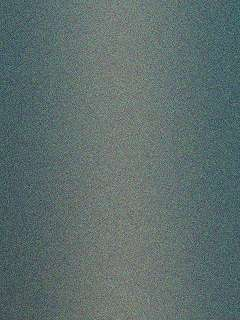
\includegraphics[height=0.25\textheight,width=0.4\textwidth]{/imageProcessing/gradeschlecht.jpg}\label{img_badSeight}}
\end{tabular}
\caption[Simulationsbilder]{Simulationsbilder. \textit{a)} zeigt das ursprüngliche Bild. In \textit{b)} bis \textit{d)} wird das Bild auf verschiedenen Arten verschlechtert. Die Testläufe wurden mit der Verschlechterung von \textit{b)} und \textit{c)} durchgeführt. Tests unter sehr schlechten Bedingungen mit einem Grad der Verschlechterung aus \textit{d)}}
\label{simPics}
\end{figure}
\newpage
\subsection{Transformation}
\label{sec_transformations}
Wie bereits in der Einleitung beschrieben, werden mehrere Koordinatensysteme genutzt. Zur sicheren Verwendung der Koordinatensysteme sind \glspl{transform} unter den Systemen zwingend nötig.
Eine \gls{transform} besteht aus einer Rotation und einer Translation, die sich aus den Beziehungen der Systeme zueinander ergibt.\\
Im \texttt{enum} \textit{frames} [Listing \ref{framesEnum}] sind die verschiedenen Frames definiert, zwischen denen eine \gls{transform} möglich ist.

\lstinputlisting[language=Matlab,inputencoding=utf8, extendedchars=true,caption={Enumeration der Frames,die die verschiedenen Koordinatensystem bezeichnen},label=framesEnum]{frames.m}

Umgesetzt wird eine \gls{transform} aus einem \textit{source} Frame in einen \textit{target} Frame durch die Funktion \texttt{transform} [Listing \ref{transform}]. Die Transformation ist nur in eine Richtung möglich, da die inverse Transformation für diese Arbeit nicht benötigt wurde.

\lstinputlisting[language=Matlab,caption={[\gls{transform} von \textit{source} in \textit{target} Frame.]\gls{transform} von \textit{source} in \textit{target} Frame. Die verschiedenen Transformation werden hier verwaltet und solange die nächste Transformation ausgeführt, bis der \textit{target} Frame erreicht wird.},label=transform]{transform.m}

\subsubsection{Bild zu Kamera}
\label{section_PicToCam}
Die verlustfreie \gls{transform} von 2D-Pixelkoordinaten in 3D-Kamerakoordinaten ist mit einer Kamera nicht möglich, da die Tiefeninformation nicht vorhanden ist. Jedoch lässt sich mit dem Wissen über die Entfernung zur Bildebene, der \textit{flat world assumption} (siehe Kapitel \ref{sec_coordsystems}) und den intrinsischen Kameraparametern eine ausreichend gute Transformation durchführen. Da die Kamera gerade nach unten gerichtet ist, entspricht die Entfernung zur Bildebene der Höhe des \gls{auv}s über dem Meeresboden, welche über die Sensorik bestimmt wird. Die intrinsischen Kameraparameter lassen sich über eine Kamerakalibrierung bestimmen, welche mithilfe der \matlab\ \textit{Computer Vision System Toolbox} durchgeführt wird.\\
Da die resultierende \gls{transform} am besten im Abstand der Kalibrierung funktioniert wurde die Kalibrierung in einem Abstand von 6 Metern durchgeführt, was im späteren Verlauf auch der gewünschte Abstand zum Boden ist.\\
Aus der Kamerakalibrierung wird ein \textit{CameraParameter}\footnote{CameraParameter Klasse: \url{https://de.mathworks.com/help/vision/ref/cameraparameters-class.html}, Abrufdatum \textit{05.01.2017}} Objekt erzeugt, welches die Methode \textit{pointsToWorld} bietet. Die Methode berechnet eine Projektionsmatrix aus den Kamera-Parametern und dem bekannten Abstand der Kamera zum Objekt. Mithilfe der Inversen dieser Matrix können dann Pixel in Kamerakoordinaten umgerechnet werden.\\
Leichte Neigungswinkel, die während der Fahrt auftreten, können durch die Multiplikation mit der entsprechenden Rotationsmatrix herausgerechnet werden. Jedoch ist dabei zu beachten, dass durch die Neigungswinkel die Fläche, die die Kamera sieht, vergrößert wird. Dadurch bilden einzelne Pixel mehr Fläche ab und die \gls{transform} wird ungenauer.\\
Die $z$-Koordinate ergibt sich aus dem Wissen, Objekte am Meeresboden zu betrachten und der Tatsache, dass die Höhe der Kamera über dem Meeresboden bekannt ist.

\subsubsection{Kamera zu Body}
Die \gls{transform} vom Kamerakoordinatensystem zum Bodykoordinatensystem besteht aus einer Translation und einer Rotation, die durch die Montageposition der Kamera am \gls{auv} bestimmt wird [Kapitel \ref{sec_img_cam_coords}].\\
Aufgrund der Verschiebung der Kamera zum Bodykoordinatenursprung (Schwerpunkt des \gls{auv}s) ergibt sich eine Translation um $1,3$ Meter in x-Richtung und $0,25$ Meter in z-Richtung.\\
Die Rotation beträgt dabei $90^\circ$ um die Z-Achse.\\
Somit ergibt sich die Tranformationsmatrix aus Gleichung \ref{trans_cam_body}\\

\begin{ownequation}[H]
\begin{equation}
\begin{pmatrix}
x_{body}\\y_{body}\\z_{body}\\1
\end{pmatrix}
=
\begin{pmatrix}
0 & -1 & 0& 1,3\\
1 & 0 & 0& 0\\
0 & 0 & 1& 0,25\\
0 & 0 & 0 & 1
\end{pmatrix}
\cdot
\begin{pmatrix}
x_{cam}\\y_{cam}\\z_{cam}\\1
\end{pmatrix}
\end{equation}
\caption[\gls{transform} der Kamerakoordinaten zu Bodykoordinaten]{Transformation der Kamerakoordinaten zu Bodykoordinaten. Die Kamerakoordinaten werden um $1,3$ Meter auf der X-Achse und $0,25$ Meter auf der Z-Achse verschoben. Außerdem wird eine Rotation um $90^\circ$ um die Z-Achse durchgeführt.}
\label{trans_cam_body}
\end{ownequation}

\subsubsection{Body zu Welt}
Für die \gls{transform} vom Bodykoordinatensystem in das Weltkoordinatensystem ist wieder eine Translation und eine Rotation nötig.
Aus der Definition der Koordinatensysteme folgt zunächst eine Rotation um $180^\circ$ um die X-Achse.
Die Translation ergibt sich aus der Position des \gls{auv}s (Position Nord/Ost in Metern).\\
Die Rotation wird durch die Ausrichtung des \gls{auv}s in der Welt (\gls{yaw} [Abb. \ref{Abb. 2}]) bestimmt. Somit ergibt sich die Tranformationsmatrix aus Gleichung \ref{trans_body_world}\\

\begin{ownequation}[H]
\begin{equation}
\begin{split}
\begin{pmatrix}
x_{world} \\ y_{world} \\ z_{world} \\ 1
\end{pmatrix}
& =
\begin{pmatrix}
cos(yaw) & -sin(yaw) & 0 & Pos_{north}\\
sin(yaw) & cos(yaw) & 0 & Pos_{east}\\
0 & 0 & 1 & 0\\
0 & 0 & 0 & 1
\end{pmatrix}\\
&\cdot
\left(
\begin{pmatrix}
1 & 0 & 0& 0\\
0 & -1 & 0& 0\\
0 & 0 & -1& 0\\
0 & 0 & 0 & 1
\end{pmatrix}
\cdot
\begin{pmatrix}
x_{body} \\ y_{body} \\ z_{body} \\ 1
\end{pmatrix}
\right)\\
\end{split}
\end{equation}
\caption[\gls{transform} der Bodykoordinaten zu Weltkoordinaten]{Transformation der Bodykoordinaten zu Weltkoordinaten. Zunächst werden die Body-Koordinaten um $180^\circ$ um die X-Achse rotiert. Im Anschluss findet eine Translation zu der Position des \gls{auv}s in der Welt und eine Rotation um die Z-Achse, die die Ausrichtung des \gls{auv}s abbildet, statt.}
\label{trans_body_world}
\end{ownequation}

\subsubsection{Welt zu \glsentryshort{vrml}}
Für die \gls{transform} von Weltkoordinaten in \gls{vrml} Koordinaten ist nur eine Rotation um $-90^\circ$ um die X-Achse nötig [Abb. \ref{trans_world_vrml}].
\begin{ownequation}[H]
\begin{equation}
\begin{pmatrix}
x_{vrml}\\y_{vrml}\\z_{vrml}\\1
\end{pmatrix}
=
\begin{pmatrix}
1 & 0 & 0& 0\\
0 & -1 & 0& 0\\
0 & 0 & -1& 0\\
0 & 0 & 0 & 1
\end{pmatrix}
\cdot
\begin{pmatrix}
x_{body}\\y_{body}\\z_{body}\\1
\end{pmatrix}
\end{equation}
\caption[\gls{transform} von Weltkoordinaten in \glsentryshort{vrml} Koordinaten]{Transformation von Weltkoordinaten in \gls{vrml} Koordinaten. Hierfür ist nur eine Rotation um $-90^\circ$ um die X-Achse nötig.}
\label{trans_world_vrml}
\end{ownequation}
\newpage
\newpage
\subsection{Objekterkennung}
\label{sec_objDet}
%In diesem Kapitel wird die umgesetzte Objekterkennung beschrieben. Dabei wird aus einem Rohbild der Kamera ein \textit{pointInFrame}-Objekt erzeugt. Grob besteht die Objekterkennung aus zwei Schritten. Zuerst wird aus dem Rohbild ein Binärbild erzeugt und im Anschluss im Binärbild das gesuchte Objekt detektiert.
\subsubsection{Binärbild mit Template}
\label{sec_templ}
Die Objekterkennung basiert auf einem ähnlichen Verfahren wie das vorgestellte CSurvey Projekt\cite{Albiez2015CSurveyA}.\\
Da eine Farberkennung aufgrund der Sichtbedingungen nicht in Frage kommt, wird im ersten Schritt das RGB-Bild in ein Graustufenbild umgewandelt. Der erste Ansatz bestand darin das Helligkeitsbild zu betrachten, da ein gesuchtes Objekt einen höheren Helligkeitswert besitzt als der Meeresboden (siehe Abb. \ref{brightCurve_real} und \ref{brightCurve_sim}).\\
Aus Erfahrungswerten früherer Projekte riet Christopher Gaudig die Rotwerte der Bilder zu betrachten, da oftmals sowohl der Meeresboden als auch trübes Wasser geringe Rotwerte haben. In den Abbildungen \ref{redCurve_real} und \ref{redCurve_sim} ist dies zu beobachten. Die Kurven sehen denen der Helligkeitswerte sehr ähnlich, jedoch sind die Ausschläge des Objektes in den Rotwerten höher.

\begin{figure}[H]
\begin{tabular}{cc}
\multicolumn{2}{c}{\subfloat[Originalbild. Das Testbild stammt aus Aufnahmen eines Testlaufs im Unisee (siehe Abschnitt \ref{realObjTests}.]{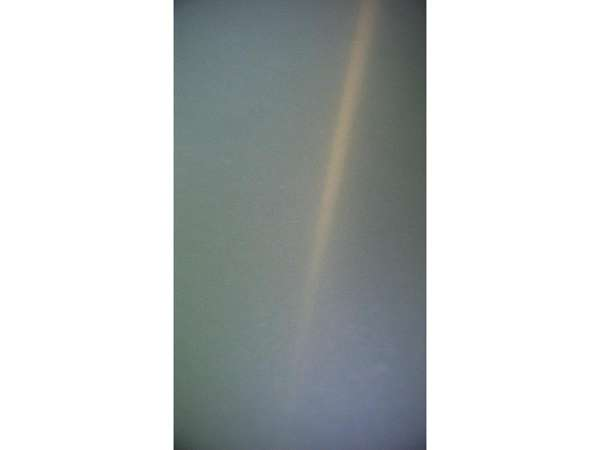
\includegraphics[height=0.2\textheight,width=\textwidth]{imageProcessing/realPipe/003orgImstart.jpg}}}\\
\subfloat[Auswertung des Helligkeitsverlauf einer Bildzeile im oberen Drittel des Bildes]{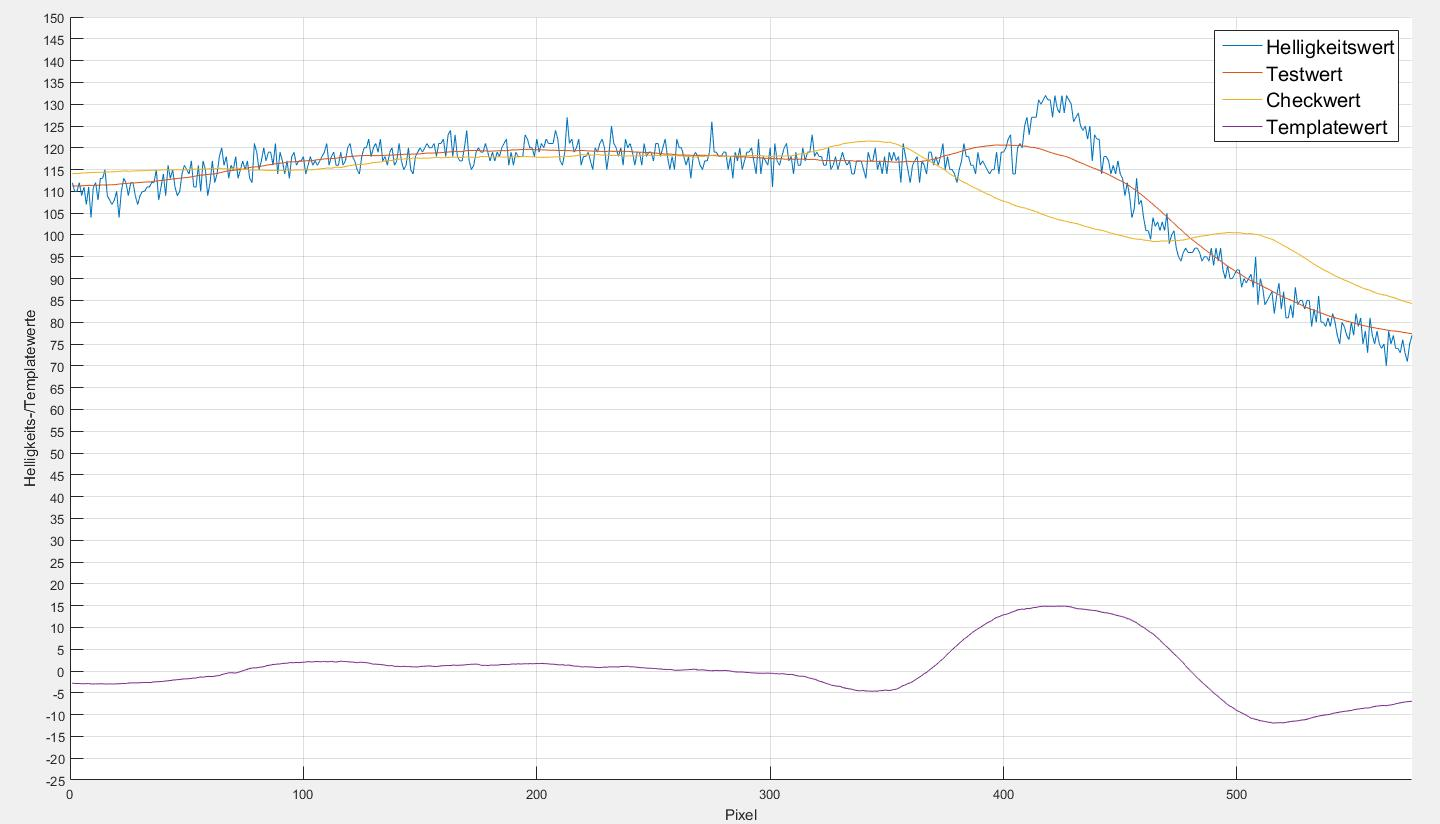
\includegraphics[height=0.2\textheight,width=0.5\textwidth]{imageProcessing/Prinzip/hellReal.jpg}\label{brightCurve_real}}&
\subfloat[Auswertung des Rotwertverlauf einer Bildzeile im oberen Drittel des Bildes]{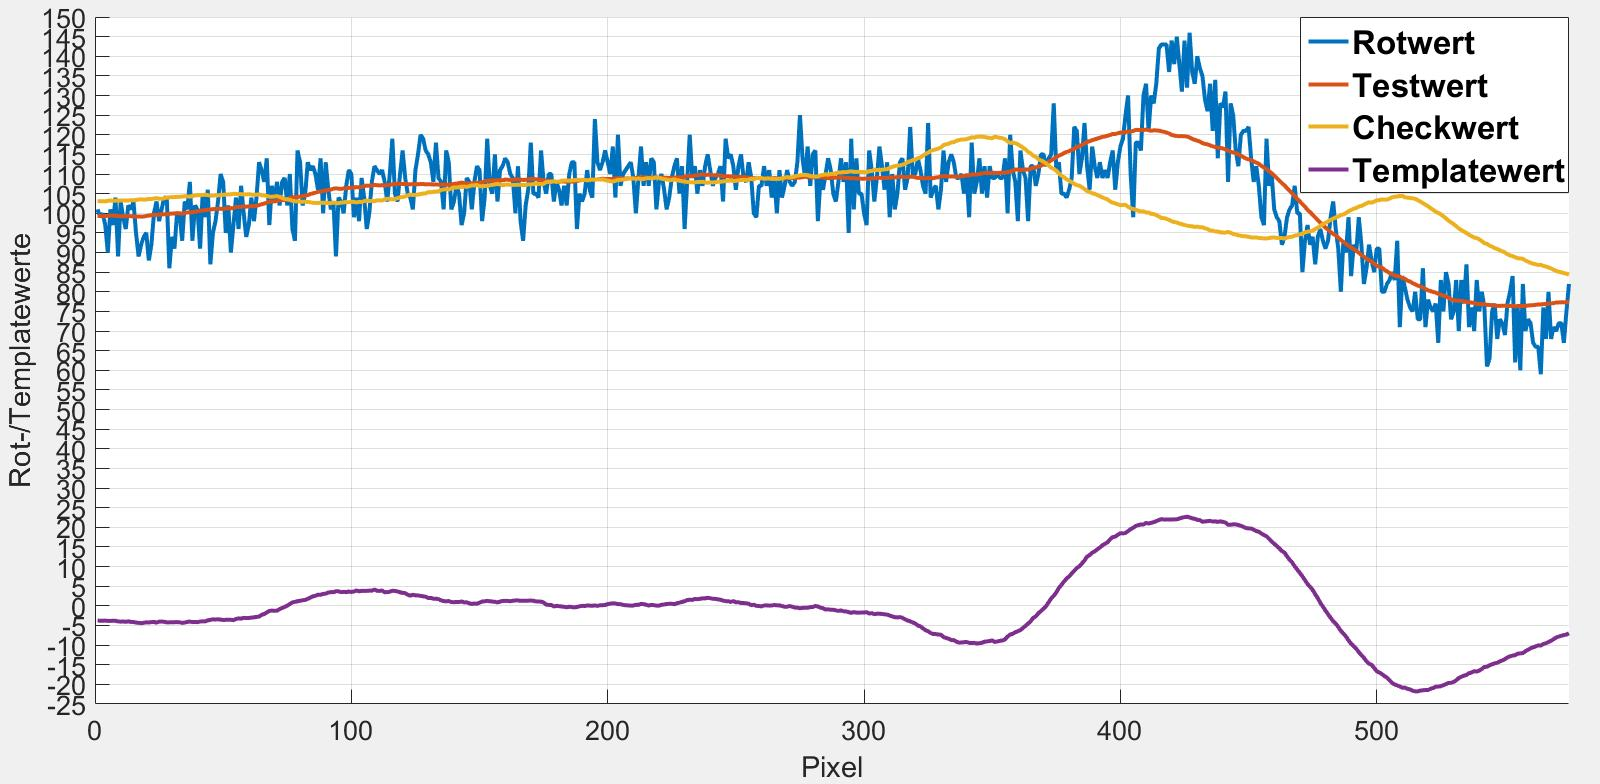
\includegraphics[height=0.2\textheight,width=0.5\textwidth]{imageProcessing/Prinzip/rotReal.jpg}\label{redCurve_real}}
\end{tabular}
\caption[Helligkeit und Rotwert im echten Testbild]{Helligkeit und Rotwert im echten Testbild. In beiden Grafiken zeigt die blaue Linie die jeweiligen Pixeldaten, die rote Linie den Wert des Testbereichs, die gelbe Linie den Durchschnitt des Checkbereichs und die weiter unten gelegene lila Linie den Templatewert für das Pixel. In beiden Templatewerten ist die Pipeline eindeutig zu erkennen, wobei der Ausschlag im Rotwert weitaus höher ist.}
\end{figure}

\begin{figure}[H]
\begin{tabular}{cc}
\multicolumn{2}{c}{\subfloat[Originalbild der Simulation]{\includegraphics[height=0.2\textheight,width=0.4\textwidth]{imageProcessing/gradeTestQuali.jpg}}}\\
\subfloat[Auswertung des Helligkeitsverlaufs einer Bildzeile im oberen Drittel des Bildes]{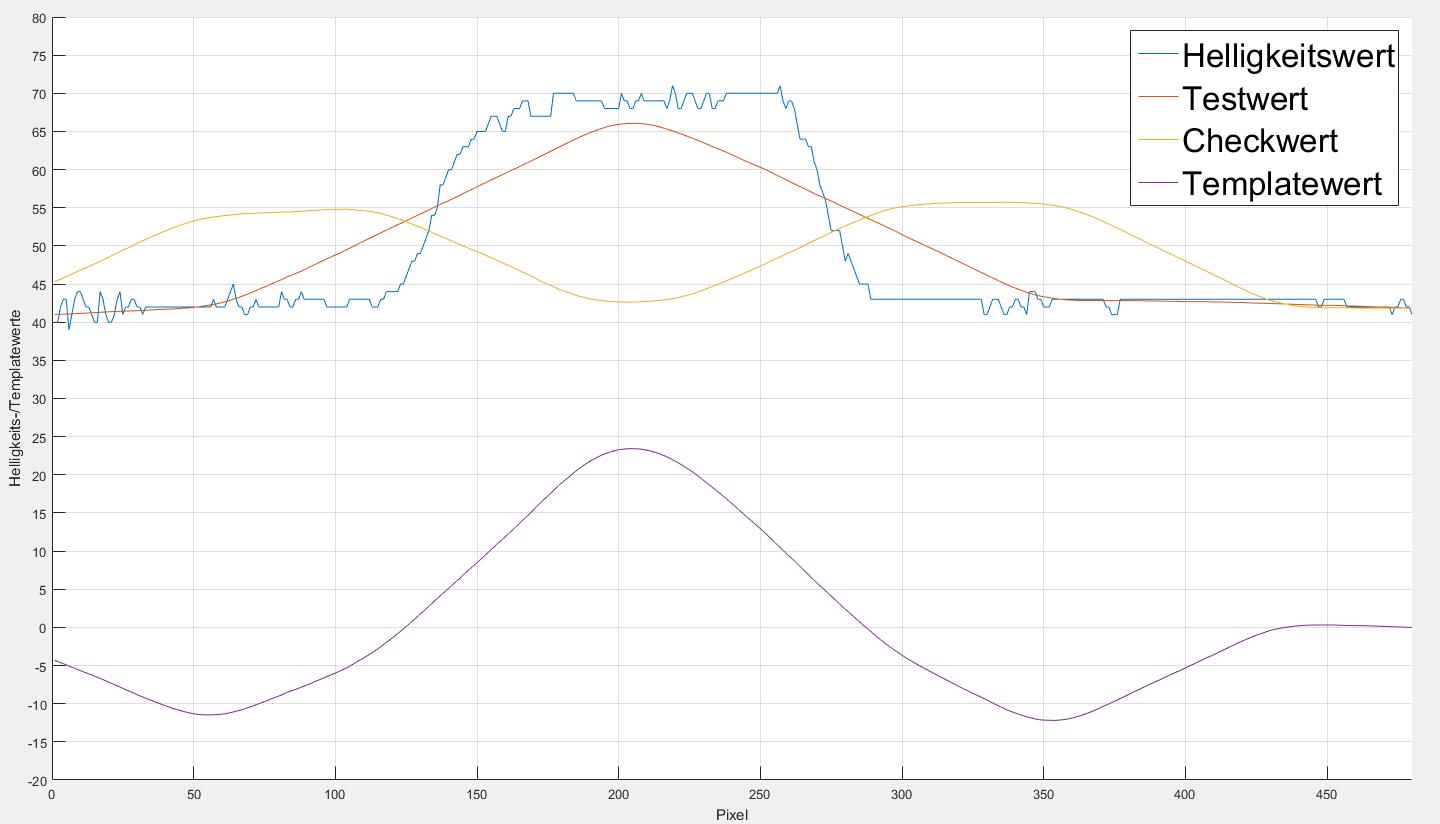
\includegraphics[height=0.2\textheight,width=0.5\textwidth]{imageProcessing/Prinzip/hellSim.jpg}\label{brightCurve_sim}}&
\subfloat[Auswertung des Rotwertverlaufs einer Bildzeile im oberen Drittel des Bildes]{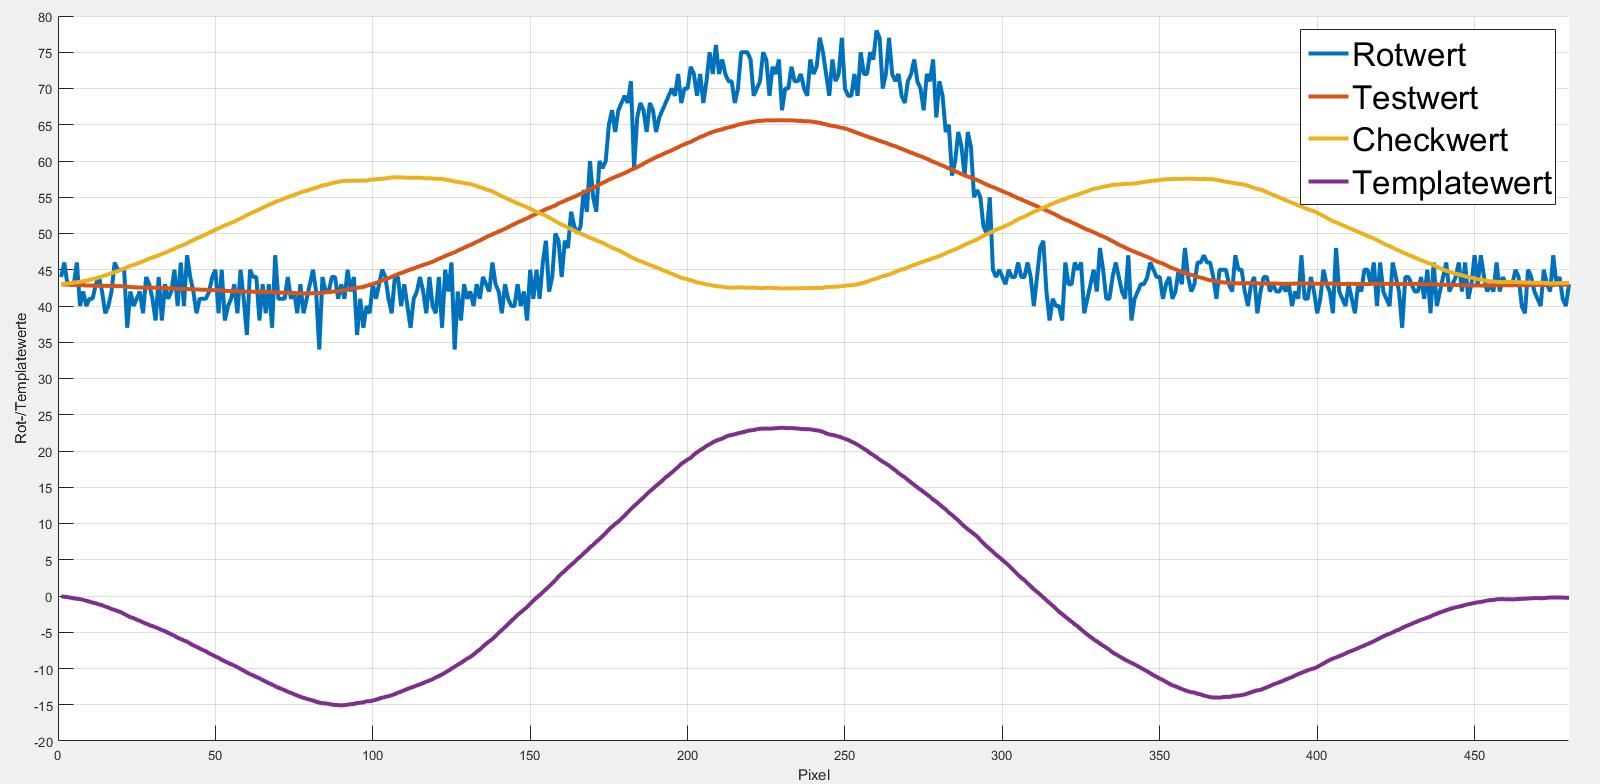
\includegraphics[height=0.2\textheight,width=0.5\textwidth]{imageProcessing/Prinzip/rotSim.jpg}\label{redCurve_sim}}
\end{tabular}
\caption[Helligkeit und Rotwert im Simulationsbild]{Helligkeit und Rotwert im Simulationsbild.In beiden Grafiken zeigt die blaue Linie die jeweiligen Pixeldaten, die rote Linie den Wert des Testbereichs, die gelbe Linie den Durchschnitt des Checkbereichs und die weiter unten gelegene lila Linie den Templatewert für das Pixel. In beiden Templatewerten ist die Pipeline eindeutig zu erkennen, wobei der Ausschlag im Rotwert weitaus höher ist.}
\end{figure}
Im nächsten Schritt wird mithilfe eines Templates [Abb. \ref{templImg}] ein Binärbild erzeugt. Das Template zeichnet sich durch drei Pixelangaben aus. Die \textit{Testpixel} (rot) geben einen Bereich an, der im aktuellen Schritt geprüft wird. Die \textit{Checkpixel} (blau) geben den Bereich rechts und links neben dem Testbereich an und bilden den Referenzwert. Die \textit{Borderpixel} (grün) geben einen Bereich zwischen Test- und Checkbereich an, der ignoriert wird.

\begin{figure}[H]
\centering
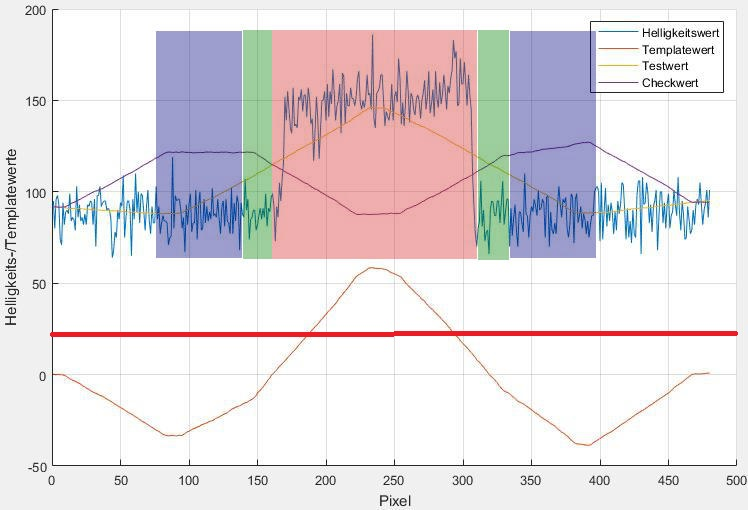
\includegraphics[height=0.3\textheight,width=\textwidth]{imageProcessing/Prinzip/template.jpg}
\caption[Template zum Bestimmen des Binärbilds]{Template zum Bestimmen des Binärbilds. Getestet wird das Pixel im Zentrum des Testbereichs (rot). Der Templatewert ergibt sich aus der Subtraktion des Durchschnitts im Checkbereich (blau) vom Durchschnitt des Testbereichs (rot). Der Borderbereich (grün) wird dabei nicht beachtet. Die rote Linie stellt den Templateschwellenwert dar, der überschritten werden muss.}
\label{templImg}
\end{figure}

Durch das Ignorieren des Borderbereichs kann ein langsamer, regelmäßiger Übergang einen hohen Templatewert in den zum Objekt gehörenden Pixeln ergeben. Ohne diesem Bereich zwischen Test- und Checkbereichs würde dies zu einem geringen Templatewert in allen Pixeln führen.\\
Die Breite des Testbereichs entspricht der erwarteten Breite des Objektes im Bild. Der Checkbereich ist dabei halb so groß und der Borderbereich wird konstant auf $10$ Pixel gesetzt. Dieser Wert führt im Zielabstand zum Boden, der in dieser Arbeit genutzt wird, zu einem ausreichend breiten Bereich.\\
Jedes Pixel dient einmal als Mittelpunkt des Testbereichs, um zu entscheiden, ob das betrachtete Pixel Teil des Objektes sein kann. Dies ist der Fall, wenn der Wert des Pixels [Gleichung \ref{templateValue}] einen Schwellenwert (rote Linie in Abb. \ref{templImg}) übersteigt.\\

\begin{ownequation}[H]
\begin{equation}
TV = \frac{sum(Testpixel)}{\#TP} - \frac{sum(Checkpixel)}{\#CP}
\end{equation}
\caption[Templatewertberechnung für ein Pixel als Formelausdruck]{Templatewertberechnung für ein Pixel als Formelausdruck.Der berechnete Wert $TV$ ist der Unterschied zwischen Test- und Checkbereich.$\#TP$ bezeichnet die Anzahl der Testpixel und $\#CP$ die Anzahl der Checkpixel.}
\label{templateValue}
\end{ownequation}

\newpage
\subsubsection{\gls{rans} auf Binärbild}
Im weiteren Verlauf wird auf dem  Binärbild gearbeitet. Nach dem Vorbild von Wang et al. \cite{wang2004lane} wird das Bild in drei Segmente unterteilt.\\
In jedem Segment wird dann mithilfe des \gls{rans}-Algorithmus ein Rechteck gesucht [Listing \ref{ransPseudo}]. Der Algorithmus sampled verschiedene Rechtecke im Segment. Jedes Rechteck wird durch einen Mittelpunkt, eine Orientierung, die Breite und die Höhe definiert. Die Höhe ergibt sich aus der Höhe des Segmentes und die Breite wird durch die erwartete Breite des Objektes festgelegt. Mittelpunkt und Orientierung werden in jedem Iterationsschritt zufällig gewählt.\\
Für jeden Punkt des Binärbilds wird dann geprüft, ob er im Rechteck liegt (ein \textit{Inlier} ist). Gemäß des \gls{rans} wird das Rechteck mit den meisten Inliern gewählt.\\
\begin{lstlisting}[language=Matlab,caption={Eingesetzter \gls{rans} als Pseudocode.},label=ransPseudo]
function ransac(segment,height,width,minInlier,iterNum)
	maxInlier = 0;
	orientations = -pi/4:0.05:pi/4;
	bestCenter = None;
	bestOrientation = None;
	for i = 1:iterNum
		boxCenter = selectRandomPoint(segment);
		boxOrientation = selectRandomValue(orientations);
		inliers = findPointsInBox(segment, box=[boxCenter,boxOrientation,height,width]);
		
		if(len(inliers) > minInlier && len(inliers) > maxInlier)
			maxInlier = len(inliers)
			bestCenter = boxCenter;
			bestOrientation = boxOrientation;
		end
	end
end
\end{lstlisting}

Somit gibt es für jedes Bild bis zu drei Objektposen. Durch das Unterteilen in Segmente lässt sich zum einen bestimmen, in wie vielen Segmenten ein Objekt erkannt wurde (entspricht der \textit{Länge} des Objektes im Bild). Des weiteren kann ein gebogener Verlauf oder ein abgeknicktes Objekt im Bild sinnvoll erkannt werden.\\
In den ersten Tests dieses Verfahrens ist ersichtlich geworden, dass es einen Tradeoff zwischen Geschwindigkeit und Erkennungsgüte gab. Die Erkennung wurde besser, je größer das Maximum der Iteration für \gls{rans} gewählt wurden. Da der \gls{rans} jedoch auf jedes der drei Segmente separat angewendet wird, reduziert sich die Geschwindigkeit bei steigender Iterationsanzahl deutlich. Für eine zuverlässige Erkennung waren zu viele Iterationen nötig, sodass das Verfahren nicht einsetzbar wäre.\\
Als Lösung für dieses Probleme werden die möglichen erzeugten Rechtecke für den \gls{rans} begrenzt. Da das Template nur in horizontaler Richtung auf das Bild angewendet wird, sind horizontal liegende Objekte im Binärbild nicht sichtbar. Aufgrund dieser Tatsache lassen sich die Orientierungen auf einen Bereich begrenzen, anstatt diese komplett zufällig zu wählen. Durch diese Maßnahme wurden die benötigten Iterationen für ein zuverlässiges Ergebnis drastisch reduziert. Jedoch steigt auch die Gefahr Orientierungen nicht mehr richtig zu erkennen, wie in Abbildung \ref{detecFail} gezeigt.\\
\begin{figure}[H]
\centering
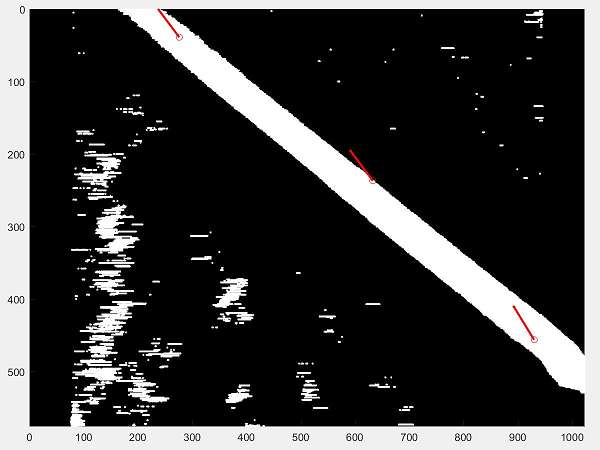
\includegraphics[scale=0.5]{imageProcessing/realPipe/004detectedImage.jpg}
\caption[Orientierung aufgrund von Beschränkung des \gls{rans} falsch detektiert]{Falsch detektierte Objektorientierung aufgrund der Beschränkung der Ausrichtungen für den \gls{rans}.}
\label{detecFail}
\end{figure}

Der zweite Faktor, der die Geschwindigkeit der Objekterkennung verringerte, ist die Menge der Punkte im Binärbild. So musste für jede Iteration des \gls{rans} für jeden Punkt geprüft werden, ob der Punkt im Rechteck liegt. In den Testbildern der Simulation lag die Anzahl der Punkte teilweise bei weit über $10000$, was in Kombination mit $200$ Iterationen zu einer inakzeptablen Laufzeit von ca. 5 Sekunden pro Bild führte.\\
Zum Lösen dieses Problems wurde vor dem Einsatz des \gls{rans} die Punktanzahl verringert, indem nur jedes dritte Pixel betrachtet wird und dieses den Mittelwert aller seiner Nachbarpixel erhält. Somit konnte die Punktanzahl zuverlässig auf unter $2000$ verringert werden, was zu einer deutlichen Beschleunigung (ca. 1 Sekunde pro Bild) ohne nennenswerte Verschlechterung der Ergebnisse führte. Die Laufzeit wurde dabei mit dem \matlab\ \textit{Stopwatch Timer}\footnote{Stopwatch Timer: \url{https://de.mathworks.com/help/matlab/ref/tic.html}, Abrufdatum \textit{05.01.2017}} gemessen.
%\subsubsection*{Gewicht der erkannten Punkte}
%\label{sec_weights}
%\begin{itemize}
%\item \textbf{numParts:} Länge des Objektes im Bild. Die erkannten Punkte werden nach Parallelität ihrer Ausrichtung und Nähe zueinander untersucht. Somit wird untersucht in wievielen Segmenten das Objekt fortgeführt wird.
%\item \textbf{area:} Um den Punkt wird ein Rechteck gelegt, dass der Breite des Objektes und der Höhe des Segmentes entspricht. \textbf{area} gibt einen relativen Wert an, wie ausgefüllt dieses Rechteck ist.
%\item \textbf{peakheight:} Es wird der Mittelwert aller der Helligkeit innerhalb des Rechtecks berechnet und mit dem allgemeinen Helligkeitswert des Bildes verglichen. \textbf{peakheight} dieses Verhältnis relativ an.
%\item \textbf{fitsBorder:} Gibt als boolean an, ob das erkannte Objekt der berechneten Objektbreite passt.
%\item \textbf{relativeCount:} Gibt das Verhältnis von Punkten im Binärbild, die zum Objekt passen und der Gesamtzahl der Punkte an.
%\end{itemize}
\newpage
\subsection{Schätzverfahren}
\label{sec_curveFit}
In diesem Abschnitt wird das implementierte Schätzverfahren erläutert. Das Verfahren nutzt die Ergebnisse der Bilderkennung und versucht mithilfe der Regression ein Polynom $f$ zweiten Grades durch alle erkannten Punkte unter Betrachtung ihrer Orientierung zu fitten. Da von geringen Krümmungsgraden der Objekte ausgegangen wird bildet eine Polynom zweiten Grades ein gutes Modell der Objekte. Mit einer Geraden wäre es nicht möglich auch nur den leichtesten Krümmungsgrad angemessen abzubilden. Polynome höheren Grades haben in diesem Anwendungsfall das Problem leicht zu \textit{kurvig} zu extrapolieren. Im Bereich der detektierten Punkte können auch solche Polynome gute Ergebnisse liefern, im Bereich danach jedoch sehr leicht mit starker Krümmung abfallen. Außerdem wäre der Parameterraum für die Regression mit jedem höheren Grad erhöht, ohne einen Mehrwert zu bieten.\\
Der Ansatz basiert auf dem \textit{Least-Squares} Verfahren\cite{simon2006optimal}, wobei versucht wird, die Gleichung \ref{lsq} zu minimieren.
$x_i$ und $y_i$ sind hierbei die Koordinaten der erkannten Punkte. Es wird über alle Punkte der quadratische Fehler vom Funktionswert für ein $x$ zu gegebenen Modellparametern $p$ zum $y$ aus der Bilderkennung summiert. $f(p,x)$ ist eine beliebige Funktion, die $x$ in Abhängigkeit von $p$ auf eine reelle Zahl abbildet.\\
\begin{ownequation}[H]
\begin{equation}
err = \sum_{i}(f(p,x_i)-y_i)^2
\end{equation}
\caption[Least-Squares-Ansatz]{Least-Squares-Ansatz. $x_i$ und $y_i$ sind die erkannten Objektpositionen.}
\label{lsq}
\end{ownequation}
Über die Zeit gesehen wird die Menge an detektierten Punkten immer größer. Da das Ziel des Verfahrens die Vorhersage des Objektverlaufs ist, ist eine gute Extrapolation wichtiger als das richtige Abbilden aller Punkte der Vergangenheit. Für die Extrapolation ist anzunehmen, dass neuere Punkte für den Verlauf wichtiger sind als ältere. Aus diesem Grund werden die Punkte über die Zeit exponentiell aufsteigend gewichtet. Somit erhalten aktuelle Punkte einen höheren Stellenwert als ältere, ohne jedoch alte Punkte komplett zu verwerfen.\\
Um diese Anforderungen umzusetzen wird eine Erweiterung des \textit{Least-Squares} verwendet, den \textit{Weighted-Least-Squares}[Gleichung \ref{wlsq}]\\
\begin{ownequation}[H]
\begin{equation}
err = \sum_{i}w_i \cdot (f(p,x_i)-y_i)^2
\end{equation}
\caption[Weighted-Least-Squares-Verfahren]{Weighted-Least-Squares Verfahren. Erweitert das Least-Squares Verfahren um eine Gewichtung der Punkte.}
\label{wlsq}
\end{ownequation}
\newpage
Das \textit{Weighted-Least-Squares} Verfahren bietet eine gute Grundlage für die Regression. Es bleiben jedoch noch einige Probleme, die das Verfahren in der Form nicht lösen kann.
\begin{enumerate}
\item Beachtung der Orientierung erkannter Punkte
\item Bedingungen für die Kurve (z.B. maximale Steigung)
\item Schätzungen für Punktverläufe, die sich nicht durch ein einzelnes Polynom darstellen lassen
\end{enumerate}

Zum Lösen der ersten zwei Probleme bietet die \matlab -Funktion \textit{fmincon}\footnote{https://de.mathworks.com/help/optim/ug/fmincon.html} aus der Optimization Toolbox eine geeignete Lösung. Die Funktion bietet die Möglichkeit eine Funktion $F(p)$ zu minimieren, wobei mit $c(p) \leq 0$ eine Bedingung erfüllt werden muss. Die Funktion $c(p,x_i)$ [Gleichung \ref{constraint}] berechnet über den Funktionsverlauf von $f(p,x)$ mithilfe der Ableitung $f'(p,x)$ die Steigung in jedem Punkt $x_i$. Da \textit{fmincon} prüft, ob die Bedingungsfunktion kleiner 0 ist wird von der Steigung ein Maximalwert ($max_{slope}$) abgezogen (\textit{Erfüllt 2.}).\\
\begin{ownequation}[H]
\begin{equation}
c(p,x_i) = f'(p,x_i)-max_{slope}
\end{equation}
\caption[Funktion zum Überprüfen ob die Steigung einen Maximalwert nicht übersteigt.]{Funktion zum Überprüfen, ob die Steigung einen Maximalwert nicht übersteigt. $max_{slope}$ gibt die maximal erlaubte Steigung des Polynoms an, die mit der Ableitung der Funktion überprüft wird.}
\label{constraint}
\end{ownequation}
Die Funktion $F(p)$ wird als $F(p,x,y,s,w,n,m,tau)$ [Gleichung \ref{minimizeFunction}] definiert, wobei $x$ und $y$ erneut die Punkte der Bilderkennung darstellen, $s$ die erkannte Orientierung im Punkt und $w$ das Gewicht darstellt. Die Funktion $F$ besteht aus einer Linearkombination der Funktionen $g$ und $h$, wobei $g$ den summierten Fehler der Position [Gleichung \ref{posError}] ($x$,$y$ Koordinaten) und $h$ den summierten Fehler der Orientierung [Gleichung \ref{orienError}] mithilfe des \textit{Weighted-Least-Squares} Verfahren berechnen (\textit{Erfüllt 1.}). $n$ und $m$ gewichten, wie stark die einzelnen Fehlerarten (Position und Orientierung) in den Gesamtfehler für die gegebenen Funktionsparameter $p$ eingehen.\\
Um die erhaltenen Polynome einschränken zu können, wurde $F$ noch gemäß der \textit{Tikhonov Regularisierung} \cite{kaipio2006statistical} angepasst. Durch die \textit{Tikhonov-Regularisierung} können wenig gekrümmte Kurven bevorzugt werden, was für einen ruhigeren Fahrtverlauf sorgen kann.
\begin{ownequation}[H]
\begin{equation}
\label{minimizeFunction}
F(p) = F(p,x,y,s,w,n,m,tau) = n \cdot g(p,x,y,w) + m \cdot h(p,x,s,w) + tau \cdot p
\end{equation}
\begin{equation}
\label{posError}
g(p,x,y,w) = \sum_{i} w_i \cdot (f(p,x_i)-y_i)^2
\end{equation}
\begin{equation}
\label{orienError}
h(p,x,s,w) = \sum_{i} w_i \cdot (f'(p,x_i)-s_i)^2
\end{equation}
\caption[Definition der Funktion F, die im Schätzverfahren minimiert wird.]{Zusammensetzung der Funktion F, die minimiert wird. In (\ref{posError}) wird der \textit{Weighted-Least-Squares} auf den Fehler der Position und in (\ref{orienError}) auf den Fehler der Steigung angewendet.}
\label{F-function}
\end{ownequation}
\newpage
Um das Problem 3. zu lösen, betrachten wir Abbildung \ref{prob3}. Das Objekt ist hierbei so gelegen, dass das Polynom nur sehr schlecht durch die Daten gelegt werden kann und außerdem ein Teilabschnitt annähernd parallel zur Y-Achse verläuft. Der letzte Fall ist zu beachten, da ein solcher Verlauf durch eine unendliche Steigung im Polynom abgebildet werden müsste.\\
Als Lösung für dieses Problem wird ein alternatives Weltkoordinatensystem eingeführt. Dieses unterscheidet sich durch eine \gls{transform} vom echten Weltkoordinatensystem. In Abbildung \ref{prob3solved} ist zu sehen, wie durch eine \gls{transform} ein weitaus besseres Polynom für die gleichen Punkte gefunden werden kann.\\
\begin{figure}[H]
\centering
\begin{tabular}{cc}
\subfloat[Die detektierten Punkte sind so gelegen, dass das Polynom nur sehr schlecht durch die Daten gelegt werden kann.]{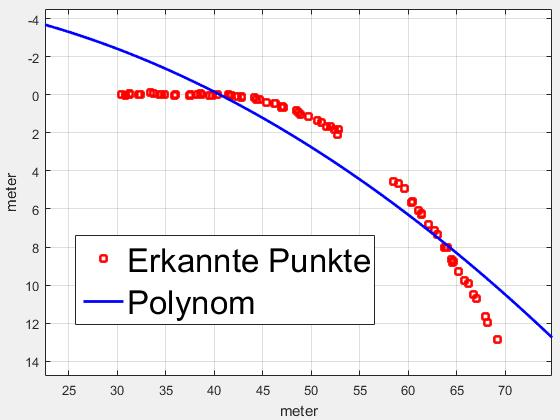
\includegraphics[scale=0.55,width=0.45\textwidth]{curveFitting/bevoreTrans.jpg}\label{prob3}}&
\subfloat[Durch die Transformation wird ein deutlich besseres Polynom gefunden.]{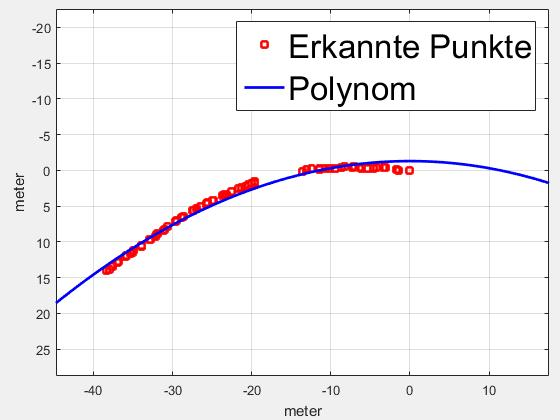
\includegraphics[scale=0.55,width=0.45\textwidth]{curveFitting/afterTrans.jpg}\label{prob3solved}}
\end{tabular}
\caption[Transformation in alternatives Koordinatensystem]{Eine Transformation der detektierten Punkte in das alternative Koordinatensystem, um ein besseres Polynom bestimmen zu können. Das Polynom in \textit{a)} übersteigt den Fehlerschwellenwert und löst damit die Transformation aus.}
\label{figAlterCoords}
\end{figure}
Nach jeder Regression wird das berechnete Polynom in den aktuellsten Punkten getestet. Sollte dabei ein gewisser Fehlerschwellenwert überschritten werden, wird eine neue \gls{transform} berechnet (vgl. Listing \ref{transPseudo}). Diese neue Transformation besteht aus einer Translation zum Punkt mit dem größten $x$-Wert und einer Rotation um die durchschnittliche Ausrichtung der neuesten Punkte. Neben der Transformationsmatrix wird auch die Inverse der Matrix gespeichert, die für die Wegpunktberechnung [Kapitel \ref{sec_waypoint}] wichtig ist. Da die Transformation ausgelöst wird, sobald das Polynom in den neuesten Punkten einen zu großen Fehler ergibt, werden nach dem Speichern der Matrizen alle Punkte, bis auf die neuesten, verworfen, um ein potentiell besseres Polynom für die Extrapolation zu ermöglichen. Die \textit{aktuellsten} Punkte wurden im Rahmen dieser Arbeit auf konstant 10 Punkte gesetzt. Bei einer größeren Anzahl an Punkten, die nach einer neuen Transformation nicht verworfen werden, konnte oftmals kein neues Polynom gefunden werden, dass die maximale Fehlerschwelle wieder unterschreitet.\\
Sobald eine beschriebene \gls{transform} gespeichert wurde, werden alle Punkte vor der Regression in das alternative Koordinatensystem transformiert. Durch diese Transformation sind die erkannten Punkte entlang der X-Achse gelegen und somit ist es möglich, stets ein geeignetes Polynom für die Punkte zu finden. Durch die Translation liegen die Punkte stets nah am Ursprung, was den Parameterraum für die Regression verringert und somit zu schnelleren Ergebnissen führt.\label{alterWorldCoords}
\begin{lstlisting}[language=Matlab,caption=Pseudocode des Schätzverfahrens,label=transPseudo]
function polynomFit(points,maxError)
	actualTransform = loadActualTransformation();
	points_T = transformPoints(points,actualTransform);
	
	polynom = regression(points_T);
	error = calculateError(points_T,polynom);
	if (error >= maxError)
		translation = findGreatestXValue(points_T);
		rotation = averageDirectionOfLastPoints(points_T);
		newTransform = createTransMatrix(-translation,-rotation) * actualTransform;
		saveNewTransform();
	end
end
\end{lstlisting}
In Listing \ref{transPseudo} ist das Schätzverfahren grob als Pseudocode dargestellt. \textit{points} ist ein Array von \textit{pointInFrame}-Objekten [Listing \ref{pointInFrame}] und \textit{maxError} gibt den Schwellenwert für eine Transformation an. Zunächst werden alle Punkte in das derzeitige alternative Weltkoordinatensystem transformiert. Sollte noch keine Transformation generiert worden sein, besteht \textit{actualTransform} aus der Einheitsmatrix und somit wird keine Transformation durchgeführt. Im Anschluss wird das Polynom durch die Regression auf den transformierten Punkten ermittelt und der Fehler in den aktuellsten Punkten berechnet. Sollte der Schwellenwert überstiegen werden wird zunächst die benötigte Translation und Rotation bestimmt und eine neue Transformationsmatrix erstellt. Diese Matrix wird mit der aktuellen Transformationsmatrix multipliziert, um beide Transformationen zu verbinden. In \textit{saveNewTransform} werden die neue Transformationsmatrix und ihre Inverse gespeichert.



